\documentclass[11pt,spanish]{article}

\usepackage[utf8]{inputenc} % Required for inputting international characters
\usepackage[T1]{fontenc}
\usepackage{mathpazo} % Palatino font
\usepackage{amsmath}
\usepackage{selinput}
\SelectInputMappings{%
	aacute={á},
	ntilde={ñ},
	Euro={€}
}
\usepackage{babel}
\usepackage{hyperref}
\usepackage{multirow}
\usepackage{caption}
\usepackage{graphicx}
\usepackage{subcaption}
\usepackage{float}
\usepackage[margin=2.5cm]{geometry}

\hypersetup{
	colorlinks,
	citecolor=black,
	filecolor=black,
	linkcolor=black,
	urlcolor=blue
}
\begin{document}
%------------------------------------------------------------------------------------------

	%---------------------------%
	%	Stop Numbering Pages	%
	%---------------------------%

	\pagenumbering{gobble}

%------------------------------------------------------------------------------------------
	\begin{titlepage} % Suppresses displaying the page number on the title page and the subsequent page counts as page 1
	
	\newcommand{\HRule}{\rule{\linewidth}{0.5mm}} % Defines a new command for horizontal lines, change thickness here
	
	\center % Centre everything on the page
	
	%---------------%
	%	Encabezados	%
	%---------------%
	
	\textsc{\LARGE Universidad Carlos III de Madrid}\\[1.5cm] % Main heading such as the name of your university/college
	
	\textsc{\Large Grado en Ingeniería Informática}\\[0.5cm] % Major heading such as course name
	
	\textsc{\large Heurística y Optimización}\\[0.5cm] % Minor heading such as course title
	
	%-----------%
	%	Titulo	%
	%-----------%
	
	\HRule\\[0.4cm]
	
	{\huge\bfseries Práctica: Programación Lineal}\\[0.4cm] % Title of your document
	
	\HRule\\[1.5cm]
	
	%---------------%
	%	Author(s)	%
	%---------------%
	
	\begin{minipage}{0.7\textwidth}
		\begin{flushleft}
			\large
			\textit{Autores}\\
			\textsc{Alberto Villanueva Nieto\ \ \ \ 100374691}\\
			\textsc{Cristian Cabrera Pinto\ \ \ \ \ \ \ \ \ \ 100363778}
		\end{flushleft}
	\end{minipage}

	%-----------%
	%	Date	%
	%-----------%
	
	\vfill\vfill\vfill % Position the date 3/4 down the remaining page
	
	{\large\today} % Date, change the \today to a set date if you want to be precise
	
	\vfill % Push the date up 1/4 of the remaining page
	
	\end{titlepage}
	\newpage
%------------------------------------------------------------------------------------------
	\tableofcontents
	\newpage
%------------------------------------------------------------------------------------------

	%---------------------------%
	%	Start Numbering Pages	%
	%---------------------------%

	\pagenumbering{arabic}

%------------------------------------------------------------------------------------------
	\section{Intorducción}
	Este documento está destinado a la explicación de los contenidos de la práctica. Esta práctica se divide en tres partes, dos partes obligatorias y una parte opcional. La primera parte se trata de un problema de satisfabilidad lógica en el cual hay que colocar a un personaje y unas serpientes en un mapa cumpliendo una serie de restricciones, para ello se explica la modelización que se ha llevado a cabo y un pequeño análisis de los resultados que se han obtenido. La segunda y tercera parte consiste en una búsqueda heurística en la que un personaje tiene que coger las llaves de un mapa, evitando las serpientes, para poder llegar a la salida. Para ello se explican la modelización que se ha llevado a cabo, las heurísticas desarrolladas y un análisis de los resultados. 
	\section{Satisfabilidad lógica}
		\subsection{Modelización}
			\subsubsection{Variables}
			\begin{itemize}
				\item Ah : Al se encuentra en el hueco h.
				\item Snh: La serpiente n se encuentra en el hueco h.
			\end{itemize}
			\subsubsection{Cláusulas}
			Para el cumplimiento de la restricción de que Al y las serpientes se encuentren tan solo en lo huecos vacíos se ha trabajado solo sobre esos huecos no teniendo en cuenta ni las paredes ni las llaves ni las rocas ni la salida.\\
			Para aclarar las siguientes cláusulas se explicaran una serie de términos:\\
			\begin{itemize}
				\item H: Conjunto de todos los huecos sobre los que se iterará con la forma (i, j). Siendo i las filas y j las columnas.
				\item h1 y h2: Hueco en el que se encuentren tanto Al como las serpientes.
				\item h1,i : Fila i del hueco h1. Para h2.i tiene el mismo significado.
				\item h1,j: Columna j del hueco h1. Para h2,j tiene el mismo significado.
				\item N: Conjunto de las serpientes que hay
			\end{itemize}
			\textbf{Un hueco por personaje}\\
			Aunque no aparece en el enunciado otra restricción que nos encotramos es que no puede haber más de un personaje en el mismo hueco. Para tratar esa restricción se crea la siguiente cláusula en la que tan solo está implicado Al (el personaje):
			\begin{equation*}
				A_{h_1} \implies \bigwedge\limits_{h_2}^H \neg A_{h_2}; h_1 \neq h_2; \forall h_1\in H
			\end{equation*}
			Esta cláusula es una implicación que itera sobre todos los huecos del mapa y significa que si Al esta el el hueco h1 no puede haber otro al en el mismo hueco pero si en otro. Además los huecos en los que esté el personaje debe pertenece al conjunto de todos los huecos del mapa.\\
			Como es una implicación no está en forma normal conjuntiva (CNF) por lo que se aplican fórmulas lógicas para llegar a ello, obteniendo la siguiente expresión para las cláusulas:
			\begin{equation*}
				\bigwedge\limits_{h_2}^H (\neg A_{h_1} \lor \neg A_{h_2}); h_1 \neq h_2; \forall h_1\in H
			\end{equation*}
			\textbf{Un hueco por serpiente}\\
			Otra restricción que nos podemos encontrar es que no puede haber más de una serpiente en el mismo hueco. Para tratar esa restricción se crea la siguiente cláusula en la que están implicadas las serpientes:
			\begin{equation*}
				S_{n,h_1} \implies \bigwedge\limits_{h_2}^H \neg S_{n,h_2}; h_1 \neq h_2; \forall h_1\in H; \forall n \in N
			\end{equation*}
			Esta cláusula es una implicación que itera sobre todos los huecos del mapa y significa que si la serpiente n está en el hueco h1 esta no puede estar en el hueco h2. Además los huecos en los que se encuentre la serpiente tiene que pertenecer al conjunto de huecos del mapa y la serpiente n tiene que pertenecer al conjunto de valores entre 0 y N-1. Pero para poder resolver el problema de satisfabilidad la cláusula tiene que estar en forma normal conjuntiva (CNF), de modo que el conjunto de cláusulas quedaría de la siguiente forma:
			\begin{equation*}
				\bigwedge\limits_{h_2}^H (\neg S_{n,h_1} \lor \neg S_{n,h_2}); h_1 \neq h_2; \forall h_1\in H; \forall n \in N
			\end{equation*}
			\textbf{Una serpiente por fila}\\
			Otra restricción que nos aparece en el enunciado es que tan solo puede haber una serpiente por fila. Para tratarla hemos llevado a cabo la siguiente cláusula:
			\begin{equation*}
				S_{n,h_1} \implies \bigwedge\limits_{h_2}^H \neg S_{m,h_2}; h_1.fila \neq h_2.fila; n \neq m; \forall h_1 \in H; \forall n,m \in N
			\end{equation*}
			Esta cláusula es una implicación que itera sobre todos los huecos del mapa y significa que si la serpiente n está en el hueco h1 con fila i entonces no puede haber otra serpiente m en un hueco h2 en la misma fila i. Los huecos en los que se encuentre la serpiente tiene que pertenecer al conjunto de huecos del mapa y las serpientes n y m tiene que pertenecer al conjunto de valores entre 0 y N-1. Pero para poder resolver el problema de satisfabilidad la cláusula tiene que estar en forma normal conjuntiva (CNF), de modo que el conjunto de cláusulas quedaría de la siguiente forma:
			\begin{equation*}
				\bigwedge\limits_{h_2}^H (\neg S_{n,h_1} \lor \neg S_{m,h_2}); h_1.fila \neq h_2.fila; n \neq m; \forall h_1 \in H; \forall n,m \in N
			\end{equation*}
			\textbf{Columna de la serpiente distinta a la columna de Al}\\
			También nos podemos encontrar otra restricción en el enunciado que nos indica que una serpiente no puede estar en la misma columna que Al. Para ello hemos modelado la siguiente cláusula:
			\begin{equation*}
				A_{h_1} \implies \bigwedge\limits_{h_2}^H \neg S_{n,h_2}; h_1.columna = h_2.columna; \forall h_1\in H; \forall n,m \in N
			\end{equation*}
			Esta cláusula itera sobre todos lo huecos del mapa y significa que si Al está en el hueco h1 con valor de columna j  no puede haber una serpiente n (con valores entre 0 y N-1) en un hueco h2  en la misma columna j. Los huecos en los que se encuentra Al y las serpientes pertenecen al conjunto de huecos del mapa. Para poder aplicar la resolución de satisfabilidad lógica las cláusulas tienen que estar en forma normal conjuntiva (CNF), de modo que el conjunto de cláusulas quedaría de la siguiente forma:
			\begin{equation*}
				\bigwedge\limits_{h_2}^H (\neg A_{h_1} \lor \neg S_{n,h_2}); h_1.columna = h_2.columna; \forall h_1\in H; \forall n,m \in N
			\end{equation*}
			\textbf{Fila de la serpiente distinta a la fila de Al}\\
			También nos podemos encontrar otra restricción en el enunciado que nos indica que una serpiente no puede estar en la misma fila que Al. Para ello hemos modelado la siguiente cláusula:
			\begin{equation*}
				A_{h_1} \implies \bigwedge\limits_{h_2}^H \neg S_{n,h_2}; h_1.fila = h_2.fila; \forall h_1\in H; \forall n\in N
			\end{equation*}
			Esta cláusula itera sobre todos lo huecos del mapa y significa que si Al está en el hueco h1 con valor de fila i  no puede haber una serpiente n (con valores entre 0 y N-1) en un hueco h2  en la misma fila i. Los huecos en los que se encuentra Al y las serpientes pertenecen al conjunto de huecos del mapa. Para poder aplicar la resolución de satisfabilidad lógica las cláusulas tienen que estar en forma normal conjuntiva (CNF), de modo que el conjunto de cláusulas quedaría de la siguiente forma:
			\begin{equation*}
				\bigwedge\limits_{h_2}^H (\neg A_{h_1} \lor \neg S_{n,h_2}); h_1.fila = h_2.fila; \forall h_1\in H; \forall n\in N
			\end{equation*}
			\textbf{Un único personaje en el mapa}\\
			Esta restricción no aparece de forma explicita en el enunciado pero es evidente que tan solo puede haber un Al en el mapa de juego, por ello se ha modelizado la siguiente cláusula para controlarlo:
			\begin{equation*}
				\bigvee\limits_{h}^H A_h; \forall h \in H
			\end{equation*}
			Está es una única cláusula sobre todos los posibles huecos en los que puede estar Al para que tan solo haya un Al en el mapa.
			\\
			\\
			\textbf{N serpientes en el mapa}\\
			Esta restricción no aparece de forma explicita en el enunciado pero es evidente que tan solo puede haber N serpiente en todo el mapa, pare ello se ha modelizado la siguiente cláusula para controlarlo:
			\begin{equation*}
				\bigvee\limits_{h}^H S_{n,h} ;\forall h \in H;\forall n \in N
			\end{equation*}
			Esta cláusula hace que para las n serpientes se compruebe que no hay más de N serpientes en todo el mapa.
		
		\subsection{Evaluación}
			\begin{tabular}{ |c||c|c|c|l| }
				\hline
				&\textbf{Tamaño}&\textbf{Serpientes}&\textbf{Tiempo}&\textbf{Resultado}\\
				\hline
				\hline
				\textbf{Mapa 1}&5x10&1&0.06 s&Se colocan correctamente las serpientes y Al\\
				\hline
				\textbf{Mapa 1}&5x10&2&0.07 s&Se colocan correctamente las serpientes y Al\\
				\hline
				\textbf{Mapa 1}&5x10&3&0.1 s&No satisfacible\\
				\hline
				\textbf{Mapa 2}&7x12&1&0.07 s&Se colocan correctamente las serpientes y Al\\
				\hline
				\textbf{Mapa 2}&7x12&3&0.09 s&Se colocan correctamente las serpientes y Al\\
				\hline
				\textbf{Mapa 2}&7x12&5&0.9 s&SNo satisfacible\\
				\hline
				\textbf{Mapa 3}&10x17&1&0.1 s&Se colocan correctamente las serpientes y Al\\
				\hline
				\textbf{Mapa 3}&10x17&5&0.18 s&Se colocan correctamente las serpientes y Al\\
				\hline
				\textbf{Mapa 3}&10x17&7&0.17 s&Se colocan correctamente las serpientes y Al\\
				\hline
				\textbf{Mapa 4}&17x25&1&0.22 s&Se colocan correctamente las serpientes y Al\\
				\hline
				\textbf{Mapa 4}&17x25&4&0.34 s&Se colocan correctamente las serpientes y Al\\
				\hline
				\textbf{Mapa 4}&17x25&8&0.54 s&Se colocan correctamente las serpientes y Al\\
				\hline
			\end{tabular}
			\\
			\\
			Con la tabla anterior podemos comprobar que:
			\begin{itemize}
				\item Dentro de un mismo mapa a mayor número de serpientes mayor es el tiempo que tarda en encontrar una solución esto es debido a que el número de nodos que tiene que expandir para la búsqueda de la solución es mayor. Este tiempo que tarda en encontrar una solución para un mismo mapa también se ve afectado por el tamaño del mapa puesto que a mayor tamaño mayor es la diferencia de tiempos que podemos encontrar dentro de un mismo mapa debido a que tiene que recorrer más columnas para cumplir con la restricción de que no haya más de una serpiente en la fila y que la serpiente no se encuentre en la misma columna que Al.
				\item En mapas distintos para el mismo caso también podemos comprobar que el tiempo que tarda en encontrar una solución es mayor y esto también es debido a la cantidad de nodos que tiene que expandir para encontrar la solución satisfacible.
				\item También podemos comprobar que a partir de cierto tamaño de mapa si hacemos que el número de serpientes a colocar sea mayor que el número de filas en las que se pueden colocar el programa tarda demasiado tiempo en determinar que el problema no es satisfacible, esto es debido a que tiene que realizar todas las combinaciones posibles para establecer un modelo y si el mapa es demasiado grande con gran cantidad de huecos en los que colocar tanto a las serpientes como al personaje el tiempo que tarda en realizar esta búsqueda es muy elevado.
				\item Otra cosa que podemos observar en la tabla anterior es que en los casos en los que si se ha obtenido una solución no satisfacible (ya que el tamaño del mapa lo permitía) el tiempo que tarda en ejecutar es mucho mayor que el tiempo que se tarda en ejecutar para el caso más extremo en el que hay una serpiente por fila, esto es debido a que el algoritmo de resolución tiene que hacer todas las comprobaciones posibles para encontrar un modelo que determine una solución posible para esa situación.
				\item Comprobando los resultados que se obtienen en todos los mapas se observa que Al siempre se encuentra en la última fila en la que haya un hueco y de ahí las serpientes quedan colocadas en las filas anteriores. También podemos observar que en todos los casos tanto Al como todas las serpientes aparecen en la casilla en la que pueden estar que está más a la izquierda del mapa. Estas dos situaciones son debidas a como está implementado el algoritmo de resolución para los problemas de satisfabilidad en la librería de Java utilizada.
			\end{itemize}
			Los mapas con los que se ha probado han sido anexados a la entrega y son los siguientes: \\
			\begin{figure}[h!]
				\begin{subfigure}[b]{0.45\linewidth}
					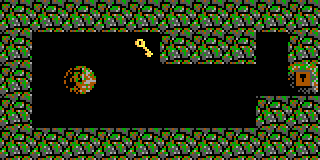
\includegraphics[width=\linewidth]{sat/lab1.png}
					\caption{Mapa 1}
				\end{subfigure}
				\begin{subfigure}[b]{0.54\linewidth}
					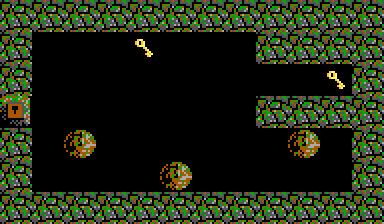
\includegraphics[width=\linewidth]{sat/lab2.png}
					\caption{Mapa 2}
				\end{subfigure}
				\begin{subfigure}[b]{0.40\linewidth}
					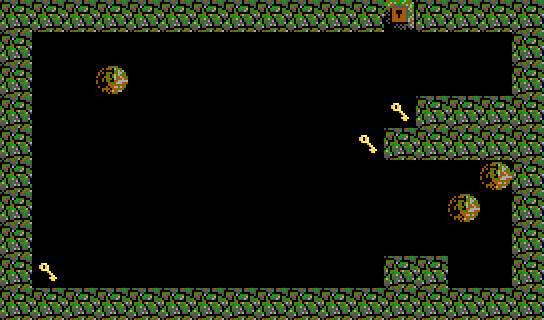
\includegraphics[width=\linewidth]{sat/lab3.png}
					\caption{Mapa 3}
				\end{subfigure}
				\begin{subfigure}[b]{0.59\linewidth}
					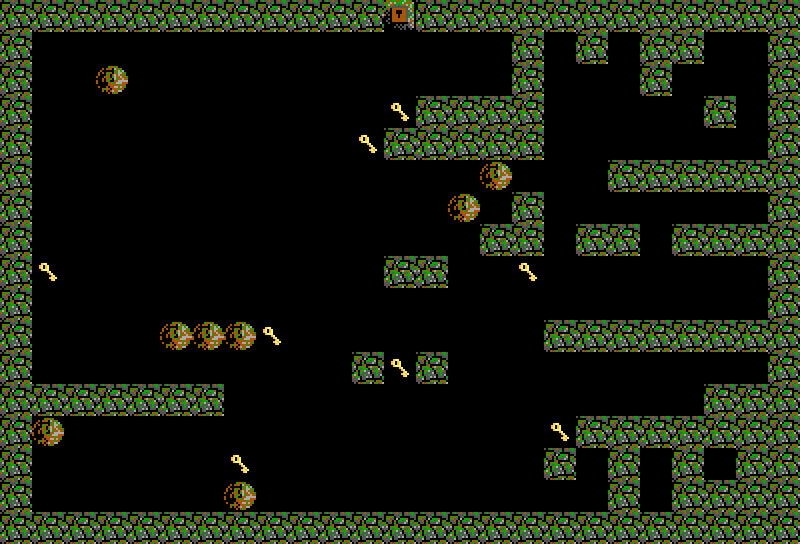
\includegraphics[width=\linewidth]{sat/lab4.png}
					\caption{Mapa 4}
				\end{subfigure}
			\end{figure}
			\\
	\section{Búsqueda heurística}
		\subsection{Modelización}
			\subsubsection{Representación de los estados}
				Dado que en los estados, lo único que es mutable es la posición de Al, la posición de las rocas, y si se han cogido o no las llaves, esto va a ser de lo único de lo que esten compuestos nuestros estados.
				\begin{itemize}
					\item Al: es la posición de Al
					\item Rocas: el conjunto formado por las posiciones de las rocas
					\item Llaves: el conjunto formado por las posiciones de las llaves que quedan\footnote{El el código se ha implementado como una lista de booleanos ya que las llaves tienen una posicion estática, de esta forma, llavesi representa si la llave i-ésima se ha recogido ($\top$ es que se ha recogido, $\bot$ es que no)}
				\end{itemize}
				Las posiciones estan representadas de la forma: (fila, columna).\\
				Y para complementarlo tendremos unos elementos globales para todos los estados:
				\begin{itemize}
					\item Muros: Conjunto con todas las posiciones a las que no se puede pasar, es decir muros, serpientes y la salida.
					\item Serpientes: Conjunto con las posiciones de las serpientes.
					\item Salida: Posicion en la que se encuentra la salida.
				\end{itemize}
			\subsubsection{Acciones y operadores}
			Al puede hacer 4 movimientos, moverse hacia arriba, hacia abajo, hacia la izquierda y hacia la derecha. Para representar los cambios que hacen el moverse en una dirección sobre al se ha representado mediante las operaciones que se hacen en las coordenadas:
			\begin{itemize}
				\item Arriba: (-1,0)
				\item Abajo: (1,0)
				\item Izquierda: (0,-1)
				\item Derecha: (0,1)
			\end{itemize}
			De esta forma, cuando escribamos arriba(al), es quivalente a disminuir la fila de al en 1.
			Para cada uno de estos movimientos, se pueden realizar dos acciones que son mutualmente exclusivas, moverse o mover una roca con coste 2 y 4 respectivamente.\\
			Además al moverse horizontalmente no hay que comprobar que haya en la fila ya que si estas en esa fila no puede haber serpientes o al estaría muerto.\\
			De esta forma las acciones y operadores quedarían definidos de la siguiente forma:\\
			\textbf{Para los movimientos verticales (Arriba y Abajo)}
			\begin{itemize}
				\item precondiciones: $(Movimiento(Al) \notin muros, rocas \land Movimiento(Al)\ no\ es peligroso) \lor (llaves = \emptyset \land Movimiento(Al) = salida)$\\
				$\implies Al = Movimiento(Al)$\\
				$\implies llaves = llaves\setminus Movimiento(Al)$
				\item precondiciones: $Movimiento(Al) \in rocas \land Movimiento(Movimiento(Al)) \notin rocas, llaves, muros$\\
				$\implies Al = Movimiento(Al)$\\
				$\implies rocas = rocas\setminus Movimiento(Al)$\\
				$\implies rocas = rocas \cup Movimiento(Movimiento(Al))$
			\end{itemize}
			\textbf{Para los movimientos horizontales (Izquierda y Derecha)}
			\begin{itemize}
				\item precondiciones: $Movimiento(Al) \notin muros, rocas \lor (llaves = \emptyset \land Movimiento(Al) = salida)$\\
				$\implies Al = Movimiento(Al)$\\
				$\implies llaves = llaves\setminus Movimiento(Al)$
				\item precondiciones: $Movimiento(Al) \in rocas \land Movimiento(Movimiento(Al)) \notin rocas, llaves, muros$\\
				$\implies Al = Movimiento(Al)$\\
				$\implies rocas = rocas\setminus Movimiento(Al)$\\
				$\implies rocas = rocas \cup Movimiento(Movimiento(Al))$
			\end{itemize}
		\subsubsection{Estado Inicial}
			El estado inicial tiene a Al, las rocas y las llaves\footnote{En nuestra implementación es un conjunto con una posicion por cada llave que hay en el mapa donde esta todo como $\bot$, ya que aun no ha recogido ninguna.} en sus posiciones iniciales.
		\subsubsection{Estado Final}
			Dado que limitamos el poder entrar en la casilla de salida para que solo entren si tienen todas las llaves, solo hay que comprobar que el estado este en la misma posicion que la salida para que sea un estado final.
		\subsubsection{heuristicas}
		Las dos heurísticas comparten 2 cosas; la funcion que usan para tomar las distancias y el coste que le añade para cubrir las serpientes que estan amenazando directamente a una llave.\\
			\\
			\textbf{Función de las distancias, dist(a,b)}\\
			Esta funcion es manhattan solo que intenta ser un poco más completa teniendo en cuenta algunos muros. La funcion se queda con el submapa conformado entre los dos puntos a y b entre los que se calcula la distancia y comprube si alguna fila o columna esta rellena por completo de muros. Si alguna fila estaba llena de muros se le suma 2 a la distancia manhattan y lo mismo para las filas. Esto se hace para indicar que Al va a tener que rodear de alguna forma ese muro.
			\begin{figure}[h!]
				\centering
				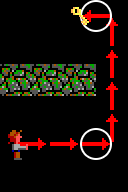
\includegraphics[width=0.2\linewidth]{Horizontal.png}
				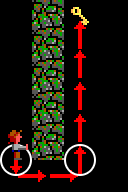
\includegraphics[width=0.2\linewidth]{Vertical.png}
				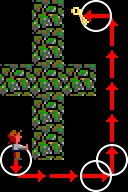
\includegraphics[width=0.2\linewidth]{HorizontalVertical.png}
			\end{figure}
			\\
			\textbf{Cubrir Serpientes, cubrir(s,k)}\\
			Esto es algo que se añade a ambas heuristicas luego el valor heurístico que devolverian las heurísticas sería $h_i = h_i'+cubrir\ serpientes$\\
			Lo que hace esta parte es comprobar todas las llaves y si alguna esta siendo directamente amenazada por una serpiente, es decir, si hay una fila en la misma fila y no hay ninguna otra llave, piedra o muro entre medias, estima un coste necesrio para cubrir la serpiente y que deje de estar amenazada.\\
			Esto se hace de la siguiente forma:
			\[
				cubrir(s,k) = 2*\min\limits_r^{rocas}
				\bigg \{
				\begin{tabular}{ll}
					$\mid k_{fila}-r_{fila} \mid $& $Si\ r_{columna} \in (s_{columna}, k_{columna})$\\
					$\min(dist(r,h_{iz}),dist(r,h_{der}))$&$ Si\ r_{columna} \notin (s_{columna}, k_{columna})$\\
				\end{tabular}
			\]
			\begin{tabular}{ll}
				k&: Posición de la llave a tapar\\
				s&: Posición de la serpiente a tapar\\
				$h_{iz}$&: El hueco inmediatamente a la derecha de la posición que esté mas \\
				&  a la izquierda entre k y s\\
				$h_{der}$&: El hueco inmediatamente a la izquierda de la posición que esté mas \\
				&  a la derecha entre k y s\\
				$k_{fila}$&: Fila de k\\
				$k_{columna}$&: Columna de k
			\end{tabular}\\
			Es decir, para cada piedra calculamos la distacia que habria que moverla para tapar la linea de vision de la serpiente a la llave, si la columna de la piedra esta entre las columnas de la llave y la serpiente solo hay que moverla hacia abajo/arriba y si esta fuera de ese rango, hay que encontrar el camino mas corto para mover la piedra hasta el limite del rango de vision que este mas cerca.\\
			Y luego lo multiplicamos por 2 para asimilarlo a los costes que se necesitan para moverse. Se usa 2 en vez de 4, que es lo que cuesta mover una roca, porque el coste añadido para mover una roca partiendo de que el movimiento se va a porducir, ya que en las heuristicas se tiene en cuenta movimiento y si aqui se usara 4, se podria estar teniendo en cuenta el coste del movimiento mas de una vez (una para el movimiento de la heuristica y otra para mover la piedra luego algo que tendria coste 4 le asignaria coste 6).\\
			\\
			\textbf{Heurística 1}\\
			Esta heurística calcula la distancia entre al y la llave mas lejana y desde la llave mas lejana hasta la salida, y si no hay llaves es la distancia desde al hasta la salida y luego lo multiplica por 2 ya que para una posicion cuesta 2.\\
			$dist(al,k_m) = \max\limits_k^{llaves}(dist(al,k))$
			\[
			h_1'
			\bigg \{
				\begin{tabular}{ll}
					$2*(dist(al,k_m) + dist(k_m,salida))$ &Si quedan llaves\\
					$2*dist(al,salida)$ &Si no quedan llaves
				\end{tabular}
			\]
			\\
			\textbf{Heurística 2}\\
			Esta heurística es muy parecida a la primera pero en vez de calcular las cosas en torno a al, las calcula en torno a la salida, es decir, primero calcula la distancia hasta la llave que esta mas lejos de la salida y luego, desde esa llave, la distancia hasta al.\\
			$dist(salida,k_m) = \max\limits_k^{llaves}(dist(salida,k))$
			\[
			h_2'
			\bigg \{
				\begin{tabular}{ll}
					$2*(dist(salida,k_m) + dist(k_m,al))$ &si quedan llaves\\
					$2*dist(salida,al)$ &si no quedan llaves
				\end{tabular}
			\]
	\subsection{Analisis}
		\subsubsection{Casos de prueba}
			Para evaluar el funcionamiento, se han usado 6 mapas distintos con las 2 heuristicas implementadas y dijkstra (f() = g()) y se han obtenido los siguientes resultados:\\
			\begin{center}
			\begin{tabular}{|c||c|c|c|}
				\hline
				\textbf{Mapa}&\textbf{Heuristica}&\textbf{Tiempo}&\textbf{Nodos Expandidos}\\
				\hline
				\hline
				\multirow{3}{*}{\textbf{Mapa 1}} & h1 & 0.001 s & 26\\
												& h2 & 0.001 s & 26\\
												& dijkstra & 0.007 s & 112\\
				\hline
				\multirow{3}{*}{\textbf{Mapa 2}} & h1 & 0.008 s & 67\\
												& h2 & 0.001 s & 81\\
												& dijkstra & 0.625 s & 1 284\\
				\hline
				\multirow{3}{*}{\textbf{Mapa 3}} & h1 & 0.021 s & 118\\
												& h2 & 0.013 s & 80\\
												& dijkstra & 501.141 s & 26 310\\
				\hline
				\multirow{3}{*}{\textbf{Mapa 4}} & h1 & 1.673 s & 2 478\\
												& h2 & 1.755 s & 2 510\\
												& dijkstra & 2.409 s & 2 806\\
				\hline
				\multirow{3}{*}{\textbf{Mapa 5}} & h1 & 34.702 s & 8 554\\
												& h2 & 29.857 s & 8 626\\
												& dijkstra & 60.447 s & 10 775\\
				\hline
				\multirow{3}{*}{\textbf{Mapa 6}} & h1 & 58.091 s & 9 097\\
												& h2 & 58.308 s & 9 251\\
												& dijkstra & 68 613.146 s & 110 372\\
				\hline
			\end{tabular}
			\end{center}
			En todos los problemas, el entorno se comporta como esperado, y se alcanza una solución óptima.
			\\
			Lo primero de todo, analizemos la complejidad para cada mapa, segun los huecos que hay libres en cada mapa y el número de rocas y llaves el número de posibles estados es el siguiente\footnote{Para el mapa 4 no se usa  la formula ya que la roca se puede ver claramente que solo puede estar en 6 posiciones}:
			$$
			nº\ estados\footnote{Realmente este no es el número real de estados, es una aproximación ya que con esta aproximacion se tiene en cuenta estados adicionales como una llave y una roca estando en el mismo sitio o al estando en una posición amenazada por una serpiente, pero es suficientemente aproximada como para hacernos una idea} = \frac{H!}{(H-(R+1))!}*2^k
			$$
			\begin{tabular}{ll}
				H &: número de huecos (incluyendo las posiciones de las rocas y de al)\\
				R &: número de rocas\\
				k &: número de llaves\\
			\end{tabular}
			\\
			Basandonos en esta formula obtenemos los siguientes números:
			\begin{center}
			\begin{tabular}{|c||c|c|c|c|c|c|c|}
				\hline
				&\textbf{H}&\textbf{R}&\textbf{k}&\pmb{$\frac{H!}{(H-(R+1))!}$}&\pmb{$2^k$}&\textbf{nº estados}\\
				\hline
				\hline
				\textbf{Mapa 1} & 23 & 1 & 1 & 506 & 2 & 1 012\\
				\hline
				\textbf{Mapa 2} & 43 & 1 & 2 & 1 806 & 4 & 7 224\\
				\hline
				\textbf{Mapa 3} & 109 & 2 & 2 & 1 259 604 & 4 & 5 038 416\\
				\hline
				\textbf{Mapa 4} & 83 & 1 & 3 & 498 & 8 & 3 984\\
				\hline
				\textbf{Mapa 5} & 39 & 2 & 2 & 54 834 & 4 & 219 336\\
				\hline
				\textbf{Mapa 6} & 78 & 2 & 4 & 456 456 & 16 & 7 303 296\\
				\hline
			\end{tabular}
			\end{center}
			Observando en esto se pueden ver ver varias cosas:\\
			\begin{itemize}
				\item La complejidad del problema crece principalmente con el número de huecos, piedras y llaves en ese orden de impacto.
				\item La salida crea una especie de muro invisible ya que en cuanto se tengan todas las llaves, suponiendo un espacio abierto, nunca se va a usar la parte del lado contrario del muro porque se llegará primero a la salida, esto se puede ver facilmente en el primer mapa ya que todos los elementos relevantes estan a la izquierda de la salida asi que si reducimos nuestros posibles estados eliminando los huecos de la parte de la derecha nos quedaría como número de posibles estados 312 que se acerca mucho más a la realidad que el 1012 estimado anteriormente luego, cuanto más cerca este la salida de los elementos pertinentes en el mapa, principalmente las llaves, antes se va a encontrar la salida, y se van a expandir menos nodos.
				\item El mapa 4 limita mucho los descendientes que se pueden crear, por ello la estimación que hemos hecho es muy similar a la expansion de nodos que hace una busqueda de fuerza bruta.
				\item La busqueda por fuerza bruta en el mapa 3 y 6 expande significantemente menos nodos que los que el numero de nodos estimados, eso es porque estos mapas contienen 2 serpientes y las serpientes hacen que muchos nodos no sean posibles y limita los sucesores que algunos nodos generan eliminando los posibles huecos que puede haber para al, luego, si aumenta el numero de serpientes la complejidad del problema disminuye siempre que siga siendo satisfacible y no aumente el numero de rocas.
			\end{itemize}
			Los mapas con los que se ha hecho el analisis han sido anexados a la entrega y son:\\
			\begin{figure}[H]
				\begin{subfigure}[b]{0.29\linewidth}
					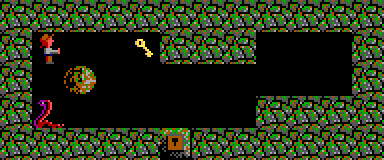
\includegraphics[width=\linewidth]{astar/lab1.png}
					\caption{Mapa 1}
				\end{subfigure}
				\begin{subfigure}[b]{0.29\linewidth}
					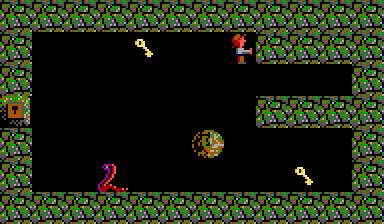
\includegraphics[width=\linewidth]{astar/lab2.png}
					\caption{Mapa 2}
				\end{subfigure}
				\begin{subfigure}[b]{0.41\linewidth}
					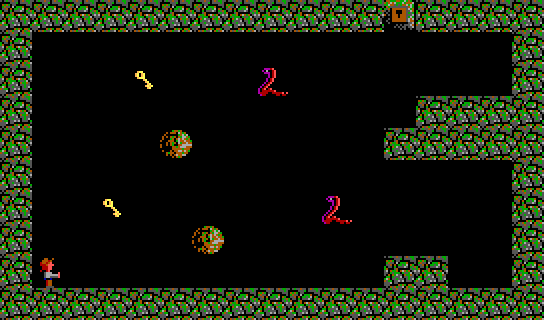
\includegraphics[width=\linewidth]{astar/lab3.png}
					\caption{Mapa 3}
				\end{subfigure}
				\begin{subfigure}[b]{0.36\linewidth}
					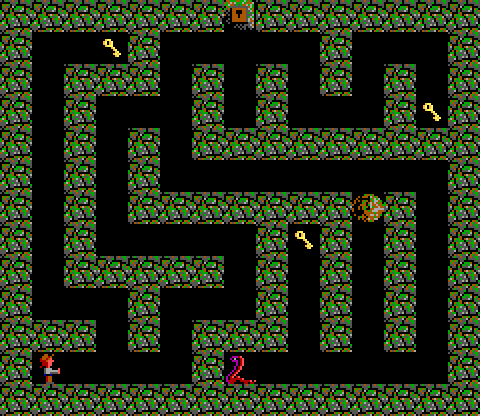
\includegraphics[width=\linewidth]{astar/lab4.png}
					\caption{Mapa 4}
				\end{subfigure}
				\begin{subfigure}[b]{0.24\linewidth}
					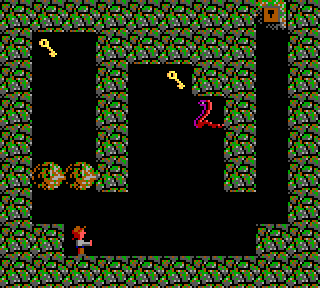
\includegraphics[width=\linewidth]{astar/lab5.png}
					\caption{Mapa 5}
				\end{subfigure}
				\begin{subfigure}[b]{0.39\linewidth}
					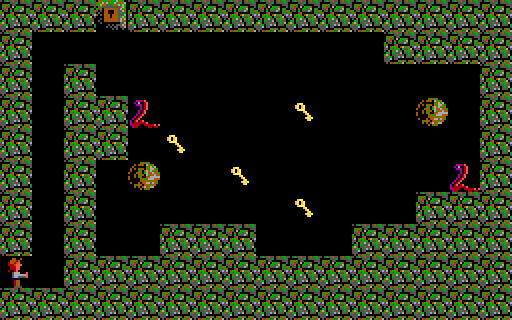
\includegraphics[width=\linewidth]{astar/lab6.png}
					\caption{Mapa 6}
				\end{subfigure}
			\end{figure}
			
		\subsubsection{Comparación de heurísticas}
	\section{Parte extra}
	Para añadir la parte adicional se han tenido que añadir movimientos en la parte de acciones y operadores y se ha cambiado una parte de las heuristicas.
		\subsection{Acciones y operadores}
			Ahora al puede hacer 4 movimientos adicionales cada uno descrito de la siguiente forma:
			\begin{itemize}
				\item arriba izquierda: (-1,-1)
				\item arriba derecha: (-1,1)
				\item abajo izquierda: (1,-1)
				\item abajo derecha: (-1,-1)
			\end{itemize}
			Y los operadores quedarian descritos como:
			\begin{itemize}
				\item precondiciones: $Movimiento(Al) \notin muros, rocas \land \neg((al_{fila},Movimiento(Al)_{columna}) \in muros \lor rocas  \land (Movimiento(al)_{fila},Al_{columna}) \in muros \lor rocas)\lor (llaves = \emptyset \land Movimiento(Al) = salida)$\\
				$\implies Al = Movimiento(Al)$\\
				$\implies llaves = llaves\setminus Movimiento(Al)$
			\end{itemize}
		\subsection{Heuristicas}
			Los cambios aqui han sido cambiar la funcion de distancias por:\\
			$$\min(f,c)-1 + \mid f-c\mid$$
			f: numero de filas entre las 2 posiciones\\
			c: numero de columnas entre las 2 posiciones\\
			\\
			Y en la funcion para calcular la distancia para mover las rocas se ha cambiado a la distancia manhattan (ya que nopuedes mover las rocas diagonalmente).\\
		\subsection{Analisis}
		\begin{center}
			\begin{tabular}{|c||c|c|c|}
				\hline
				\textbf{Mapa}&\textbf{Heuristica}&\textbf{Tiempo}&\textbf{Nodos Expandidos}\\
				\hline
				\hline
				\multirow{3}{*}{\textbf{Mapa 1}} & h1 & 0.002 s & 27\\
												& h2 & 0.002 s & 27\\
				\hline
				\multirow{3}{*}{\textbf{Mapa 2}} & h1 & 0.014 s & 73\\
												& h2 & 0.011 s & 61\\
				\hline
				\multirow{3}{*}{\textbf{Mapa 3}} & h1 & 0.835 s & 792\\
												& h2 & 1.982 s & 1 292\\
				\hline
				\multirow{3}{*}{\textbf{Mapa 4}} & h1 & 5.451 s & 4 010\\
												& h2 & 6.844 s & 4 379\\
				\hline
				\multirow{3}{*}{\textbf{Mapa 5}} & h1 & 642.194 s & 25 256\\
												& h2 & 673.194 s & 25 256\\
				\hline
				\multirow{3}{*}{\textbf{Mapa 6}} & h1 & 58.091 s & 9 097\\
												& h2 & 58.308 s & 9 251\\
				\hline
			\end{tabular}
		\end{center}
		Como se puede ver, para todos los casos se tarda más, esto es porque al haber mas posibles acciones, hay mas sucesores, muchos de los cuales se repiten, y tiene que estar haciendo muchas comprobaciones sobre cerrada y abierta para ver si cada uno de los nodos esta, ademas de calcular la heuristica varias veces mas para un mismo nodo.
	\section{Notas sobre el código}
	\begin{itemize}
		\item Para todas las partes se ha incluido un arhivo bash script llamado run.sh que se encarga de llamar al archivo correspondiente con el compilador/interprete necesario.
		\begin{itemize}
			\item parte 1: ./run.sh <laberinto>\ <n>
			\item parte 2 y opcional: ./run.sh <laberinto>\ <heuristica>
		\end{itemize}
		\item Para la parte de busqueda se ha implementado una pequeña interfaz que por defecto no esta activada, para activarla hay que cambiar el valor con el nombre de ''interfaz'' a True en el archivo config.py. Para que funcione hay que tener instalada la version de pygame para python 3.6.7
	\end{itemize}
	

%------------------------------------------------------------------------------------------

\end{document}